% ============================================================
% LLM-BLM 実験 7・8：LLM の決算の読み取りを入れた月次と日次の BLM
% コンパイル：tectonic -X compile LLM-BLM_実験7・8.tex   （XeTeX 系。このフォルダで実行する）
% 図は 図/（作成スクリプト/figs.py が experiments/E7_monthly_blm・E8_daily_blm の results から作る）
% 数値の出どころは各実験の results/summary.json と findings.md、事前登録は各実験の preregistration.md
% ============================================================
\documentclass[xelatex,ja=standard,jafont=haranoaji,a4paper,10pt,openany]{bxjsreport}
\setpagelayout*{left=24mm,right=24mm,top=24mm,bottom=26mm,footskip=11mm}

\usepackage{amsmath,amssymb,mathtools,bm}
\usepackage{booktabs,array,multirow,longtable}
\usepackage{graphicx}
\usepackage{adjustbox}
\usepackage{xcolor}
\usepackage{tikz}
\usetikzlibrary{arrows.meta,positioning,calc,fit}
\usepackage{enumitem}
\usepackage{caption}
\usepackage{float}
\usepackage[most]{tcolorbox}
\usepackage[hidelinks,bookmarksnumbered]{hyperref}
\pdfstringdefDisableCommands{\def\Omega{Ω}\def\tau{τ}\def\Sigma{Σ}}

\graphicspath{{図/}}

\definecolor{c1}{HTML}{2A78D6}
\definecolor{c2}{HTML}{EB6834}
\definecolor{c3}{HTML}{1BAF7A}
\definecolor{c4}{HTML}{EDA100}
\definecolor{c7}{HTML}{6250D6}
\definecolor{ink2}{HTML}{52514E}
\definecolor{soft1}{HTML}{E4EEF9}
\definecolor{soft2}{HTML}{FBEEDF}
\definecolor{soft3}{HTML}{E3F3E9}
\definecolor{soft4}{HTML}{EEE8FA}
\definecolor{soft5}{HTML}{FDF3DA}

\newcommand{\code}[1]{\texttt{#1}}
\newcommand{\SP}{S\&P500}
\newcommand{\figref}[1]{図~\ref{#1}}
\newcommand{\tabref}[1]{表~\ref{#1}}
\newcommand{\chapref}[1]{第~\ref{#1}~章}
\newcommand{\secref}[1]{\ref{#1}~節}

\setlist[itemize]{leftmargin=1.6em,itemsep=0.2em,topsep=0.4em}
\setlist[enumerate]{leftmargin=1.8em,itemsep=0.2em,topsep=0.4em}
\captionsetup{font=small,labelfont=bf,skip=6pt}
\renewcommand{\arraystretch}{1.2}
\setlength{\LTpre}{6pt}
\setlength{\LTpost}{6pt}

\makeatletter
\def\@makechapterhead#1{\vspace*{0.3\Cvs}{\parindent\z@\raggedright\normalfont
  \ifnum\c@secnumdepth>\m@ne\if@mainmatter{\Large\headfont\@chapapp\thechapter\@chappos}\par\nobreak\vskip0.4\Cvs\fi\fi
  \interlinepenalty\@M\LARGE\headfont #1\par\nobreak\vskip 1.5\Cvs}}
\def\@makeschapterhead#1{\vspace*{0.3\Cvs}{\parindent\z@\raggedright\normalfont
  \interlinepenalty\@M\LARGE\headfont #1\par\nobreak\vskip 1.5\Cvs}}
\makeatother

\newtcolorbox{keybox}[1][要点]{enhanced,breakable,colback=soft1,colframe=c1,boxrule=0.5pt,arc=2pt,
  left=8pt,right=8pt,top=6pt,bottom=6pt,title={#1},fonttitle=\sffamily\bfseries\small,coltitle=white}
\newtcolorbox{notebox}[1][注意]{enhanced,breakable,colback=soft2,colframe=c2,boxrule=0.5pt,arc=2pt,
  left=8pt,right=8pt,top=6pt,bottom=6pt,title={#1},fonttitle=\sffamily\bfseries\small,coltitle=white}
\newtcolorbox{verdict}[1][判定]{enhanced,breakable,colback=soft4,colframe=c7,boxrule=0.5pt,arc=2pt,
  left=8pt,right=8pt,top=6pt,bottom=6pt,title={#1},fonttitle=\sffamily\bfseries\small,coltitle=white}

\tikzset{
  box/.style={draw=#1,fill=#1!8,rounded corners=2pt,align=center,font=\footnotesize,inner sep=4pt,
              minimum height=10mm,text width=24mm},
  arr/.style={-{Stealth[length=2mm]},color=ink2,line width=0.6pt},
}

\title{LLM-BLM 実験 7・8\\[6pt]
  \large LLM の決算の読み取りを BLM に入れて、\\月次と日次でポートフォリオを組む}
\author{実験の結果の報告書}
\date{2026 年 10 月 18 日}

\begin{document}
\maketitle

% ============================================================
\chapter*{概要}
\addcontentsline{toc}{chapter}{概要}

実験 2〜4 で、gpt-4o-mini が決算発表文から読み取った点数は、発表後 2 取引日の反応を強く説明した。ただし 3 日目以降のドリフトはなかった。この報告書では、その点数を BLM の見通しに入れて、実際にポートフォリオを組んだ。

\begin{itemize}
\item \textbf{実験 7}：これまでの結果を全部入れた BLM を、月次で組んだ。
\item \textbf{実験 8}：発表日の終値の時点で、LLM の情報がまだ株価に残っているかを調べ、日次の BLM も組んだ。
\end{itemize}

2 つの実験は、手順・判定の基準・コードを同じコミット（\code{55ef830}）に固定してから、1 回ずつ実行した（事前登録）。

\begin{keybox}[主な結論]
\begin{itemize}
\item \textbf{実験 7：月次の BLM は、時価総額を有意には上回らない（支持されない）。}費用の後で月 $+0.10\%$（年 約 $+1.2\%$、$t=1.22$）。31 か月の累積は $+68.5\%$ と $+63.8\%$。実際の TE は 2.5\% と約束の 3\% 以内だった。
\item 副次の分析では、LLM の点数を銘柄の間で入れ替えた BLM を、本物が月 $+0.20\%$ 上回った（$t=2.30$）。弱い情報が月次でも残っているかもしれない。
\item \textbf{実験 8：発表日の終値の後には、LLM の情報は残っていない（支持されない）。}翌日の超過リターンへの係数は $+3.6$bp（$t=0.93$）。2 日の反応（$+116$bp）のほぼ全部が、発表日のうちに出ている。
\item \textbf{日次の BLM は費用に負ける。}毎日の最適化で 1 日に 42\% が入れ替わり、費用の後で年 $-20\%$ だった。
\end{itemize}
\end{keybox}

\setcounter{tocdepth}{1}
{\small\tableofcontents}

% ============================================================
\chapter{目的}\label{ch:intro}

これまでに分かったことを並べる。

\begin{itemize}
\item \textbf{見通しの中身}：gpt-4o-mini の点数は、決算発表への 2 日の反応を、数値の驚き・アナリスト予想・FinBERT（追加学習した版も含む）を超えて説明する（実験 2〜4）。ただし day 2〜21 のドリフトは $+10$bp で、有意でない。
\item \textbf{見通しの不確かさ $\Omega$}：LLM の 30 回の答えのばらつきは使えない（総合報告書 1）。
\item \textbf{共分散と TE}：Ledoit--Wolf で十分。TE の上限は、過去 36 か月の「実際 ÷ 予測」の比で割ると守れる（補足実験 X01〜X03）。
\end{itemize}

\begin{verdict}[問い]
\textbf{実験 7}：これらを全部入れた BLM を月次で組むと、費用の後で時価総額を上回るか。\\
\textbf{実験 8}：発表日の終値の時点で、LLM の点数は、翌日の超過リターンを予測するか。
\end{verdict}

実験 7 の予想は、実行の前に事前登録に書いた。ドリフトがなかったので、上回らない見込みが高い。株価は発表日の寄り付きで跳ねるので、日次のデータで取引できるのは、早くても発表日の終値からである。実験 8 は、そこに情報が残っているかを見る。

% ============================================================
\chapter{実験 7：月次の BLM}\label{ch:e7}

\section{設計}

\begin{table}[H]
\centering
\caption{月次の BLM の設定（事前登録で固定）。}
\small
\begin{tabular}{lp{10.6cm}}
\toprule
判断日 & 2024-01〜2026-07 の各月末（31 か月）。翌月末まで持つ。gpt-4o-mini の点数は 2023-11 以降の発表にしかないので、1 四半期分がそろう 2024-01 末から \\
銘柄 & 各月末の \SP{} の構成銘柄（平均 491） \\
事前分布 & 均衡リターン $\Pi=\delta\Sigma w_{\mathrm{mkt}}$（$\delta=2.5$） \\
見通し & 直近 92 日に反応が始まった決算発表がある銘柄（平均 454）。最新の発表の LLM の合成点数を正規スコア $z$ にし、$q_i=\Pi_i+0.05\,\sigma_i z_i$（Grinold の $\alpha$） \\
$\Omega$ & He--Litterman：$\tau\,\mathrm{diag}(P\Sigma P')$、$\tau=0.025$ \\
共分散 & 直近 252 日の Ledoit--Wolf \\
最適化 & TE の上限つきの BLM。上限は 3\% ÷ 過去 36 か月の比（X03）で、平均 1.95\% \\
取引費用 & 売買した額の 0.1\%（片道） \\
比べる相手 & 時価総額のポートフォリオ（費用なし） \\
対照 & 点数を銘柄の間で入れ替えた同じ BLM（20 通り） \\
\bottomrule
\end{tabular}
\end{table}

\section{結果}

\begin{figure}[H]
\centering
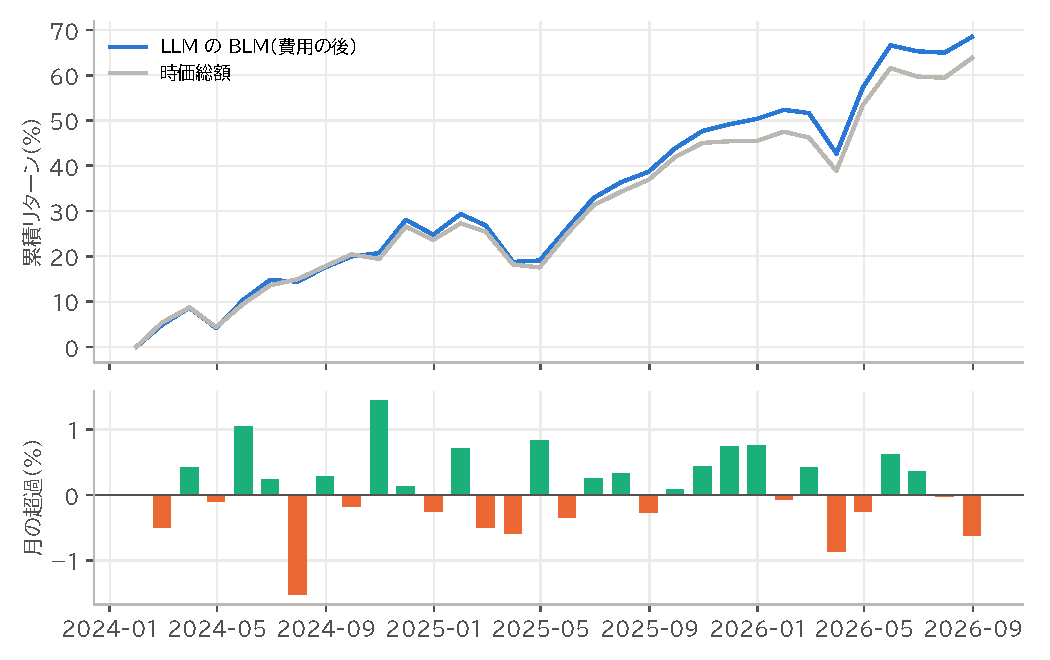
\includegraphics[width=0.92\linewidth]{e7_cumulative.pdf}
\caption{上：累積リターン（LLM の BLM は費用の後）。下：月ごとの超過リターン（緑はプラス、橙はマイナス）。}
\label{fig:e7}
\end{figure}

\begin{verdict}
\textbf{支持されない。}費用の後の超過リターンは月 $+0.10\%$、Newey--West の $t=1.22$（片側 $p=0.12$）。
\end{verdict}

\begin{table}[H]
\centering
\caption{月次の BLM の成績（31 か月）。}
\small
\begin{tabular}{lr}
\toprule
超過リターン（費用の後、月） & $+0.10\%$ \\
超過リターン（費用の前、月） & $+0.15\%$ \\
情報比（年率、費用の後） & 0.55 \\
累積（BLM ／ 時価総額） & $+68.5\%$ ／ $+63.8\%$ \\
時価総額を上回った月 & 55\% \\
回転率（月、片道） & 25\% \\
実際の TE（年率） & 2.46\% \\
\bottomrule
\end{tabular}
\end{table}

\begin{itemize}
\item 向きはプラスだが、31 か月では有意でない。事前登録に書いたとおり、この期間で検出できるのは、年率の情報比が 2 を超える場合だけである。0.55 は「ない」とも「ある」とも言えない。
\item \textbf{点数を入れ替えた対照との比較}（副次）：本物の LLM の BLM が、費用の前で月 $+0.20\%$ 上回った（$t=2.30$）。対照は費用の後で月 $-0.17\%$ と、時価総額に負けた。比率を動かすこと自体は損だが、それを上回る分が点数の中身にあった、と読める。判定に使わない分析で、期間も短いので、仮説の段階にとどめる。
\item \textbf{TE}：校正で上限が平均 1.95\% になり、実際の TE は 2.46\% と約束の内に収まった。X03 の校正は、LLM の見通しでも働いた。
\end{itemize}

% ============================================================
\chapter{実験 8：発表の翌日と日次の BLM}\label{ch:e8}

\section{第 1 部：翌日の反応（判定）}

実験 3 の標本 A（5,374 本）で、発表日（day 0）の終値から翌日（day 1）の終値までの超過リターンを、LLM の点数で回帰した。統制は実験 3 のモデル（実験 2 の統制＋アナリスト予想との差）に、day 0 の超過リターンを加えた。day 0 の終値で分かっている情報なので、LLM はそれを超える必要がある。

\begin{figure}[H]
\centering
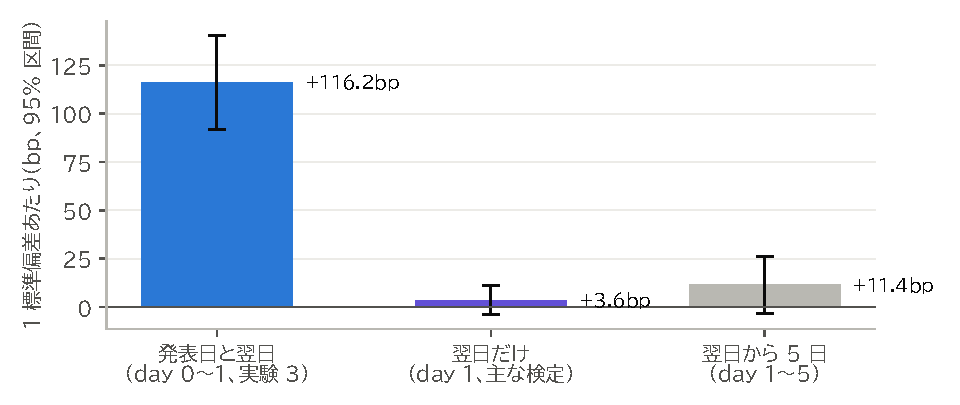
\includegraphics[width=0.86\linewidth]{e8_windows.pdf}
\caption{LLM の合成点数の係数（1 標準偏差あたり、95\% 区間）。左は実験 3 の主な結果（day 0〜1）。}
\label{fig:e8w}
\end{figure}

\begin{verdict}
\textbf{支持されない。}翌日の係数は $+3.6$bp（95\% 区間 $-4.0$〜$+11.3$、$t=0.93$、置換の $p=0.15$）。
\end{verdict}

\begin{table}[H]
\centering
\caption{翌日以降の反応への係数（1 標準偏差あたり）。}
\small
\begin{tabular}{lrrr}
\toprule
& 係数 & $t$ & $p$（片側） \\
\midrule
主な検定：day 1 & $+3.6$bp & 0.93 & 0.18 \\
S1：day 1〜5 & $+11.4$bp & 1.52 & 0.065（Holm 0.13） \\
S2：day 1（day 0 の統制なし） & $+3.4$bp & 0.87 & 0.19（Holm 0.19） \\
\bottomrule
\end{tabular}
\end{table}

\begin{itemize}
\item 2 日の反応は 1 標準偏差あたり $+116$bp だった（実験 3）。翌日に残るのは、多く見ても $+11$bp（95\% 区間の上限）で、反応のほとんどは発表日のうちに出る（\figref{fig:e8w}）。
\item day 0 の反応そのものも、翌日を予測しなかった（$-1.4$bp、$t=-0.3$）。続きも戻りもない。
\end{itemize}

\section{第 2 部：日次の BLM（報告）}

毎日、その日が発表日の銘柄にだけ見通しを付け、その終値で BLM の比率を決めて、翌日の終値まで持った。見通しの作り方と $\Omega$ は実験 7 と同じで、点数はそれより前の日の全発表で標準化した。事前の TE は 3\%、費用は片道 0.1\%。期間は 2024-04-18〜2026-08-28 の 593 取引日（過去の発表が 500 本たまった日から）。

\begin{figure}[H]
\centering
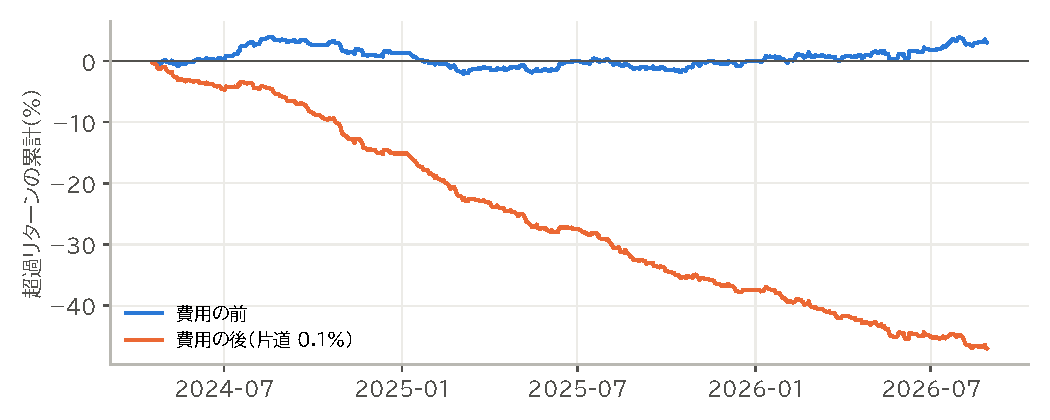
\includegraphics[width=0.92\linewidth]{e8_daily.pdf}
\caption{日次の BLM の、時価総額に対する超過リターンの累計。}
\label{fig:e8d}
\end{figure}

\begin{table}[H]
\centering
\caption{日次の BLM の成績。}
\small
\begin{tabular}{lrr}
\toprule
& LLM の BLM & 点数を入れ替えた対照 \\
\midrule
超過リターン（費用の前、年率） & $+1.3\%$ & $+2.0\%$ \\
超過リターン（費用の後、年率） & $-20.0\%$ & $-19.7\%$ \\
日次の回転率（片道） & 42\% & 43\% \\
実際の TE & 3.4\% & 3.2\% \\
\bottomrule
\end{tabular}
\end{table}

\begin{itemize}
\item 費用の前でも、LLM は対照を上回らない（差は $-0.3$bp／日、$t=-0.3$）。第 1 部と合う。
\item 毎日最適化をやり直すと、見通しのない銘柄も含めて比率全体が組み替わり、1 日に 42\% が入れ替わった。片道 0.1\% でも年 $-20\%$ になる（\figref{fig:e8d}）。日次で BLM を使うなら、売買を抑える仕組み（回転率の罰則、見通しのある銘柄だけを動かす）が欠かせない。
\item 593 日のうち 32 日は、最適化の解の精度が低い可能性があった（ソルバーの警告）。費用の前の差が対照とほぼ同じなので、結論は変わらない。
\end{itemize}

% ============================================================
\chapter{考察と限界}\label{ch:discussion}

\section{何が分かったか}

\begin{enumerate}
\item \textbf{LLM が決算発表から読み取る情報は、発表日のうちに株価に入る。}実験 2〜4 の「2 日で織り込まれる」は、実際には「発表日のうちに」だった。利益にするには、発表の直後（場中や時間外）に売買する必要があり、日次のデータでは検証できない。
\item \textbf{結果を全部入れた BLM は、約束の TE を守りながら、市場並みかやや上の成績だった。}月 $+0.10\%$ は有意でない。
\item \textbf{点数を入れ替えた対照には勝った。}月次でも弱い情報が残っているかもしれない。先読みのない ChronoGPT（実験 5）で 2016 年からの点数が作れれば、同じ BLM を約 10 年で確かめられる。
\item \textbf{日次の BLM は、設計の段階で売買を抑えないと成り立たない。}
\end{enumerate}

\section{限界}

\begin{itemize}
\item \textbf{期間が短い。}実験 7 は 31 か月、実験 8 は約 2 年 4 か月。
\item IC 0.05 は仮の値で、選び直していない。
\item 時価総額の比率は浮動株で調整していない。上場をやめた銘柄は、その後 0\% とした。
\item 標本 A は、実験 2〜5 で一度見た期間である（翌日だけの反応は見ていなかった）。
\item 日次の戦略は月ごとに並列で計算したため、月の最初の取引は時価総額の比率からの差で数えた。
\end{itemize}

% ============================================================
\chapter*{再現の手順}
\addcontentsline{toc}{chapter}{再現の手順}

\begin{verbatim}
python experiments/E2_event_reaction/run.py   # 実験 2 の panel.csv
python experiments/E7_monthly_blm/run.py      # 事前登録の後に 1 回（コミット 55ef830）
python experiments/E8_daily_blm/run.py        # 同上
cd 資料集/02_実験/実験7・8_月次と日次のBLM
python 作成スクリプト/figs.py                  # この資料の図
\end{verbatim}

数値の出どころは、\code{experiments/E7\_monthly\_blm/results/} と \code{experiments/E8\_daily\_blm/results/} の \code{summary.json}、CSV、\code{findings.md}。費用は 0 円（CPU で約 15 分）。

\end{document}
